\section{Canais de Áudio}
\label{sec:audiobus}

Canais de áudio ("audio buses") são usados para rotear sinais de áudio. É como se fossem os canais de uma mesa de som. O SuperCollider tem 128 canais de áudio como padrão. Também existem canais de controle (para sinais de controle), mas por enquanto vamos nos concentrar só nos canais de áudio.\footnote{Vamos dar uma rápida olhada em canais de controle na seção \ref{sec:control-buses}.}

\begin{figure}[h!]
\centerline{
	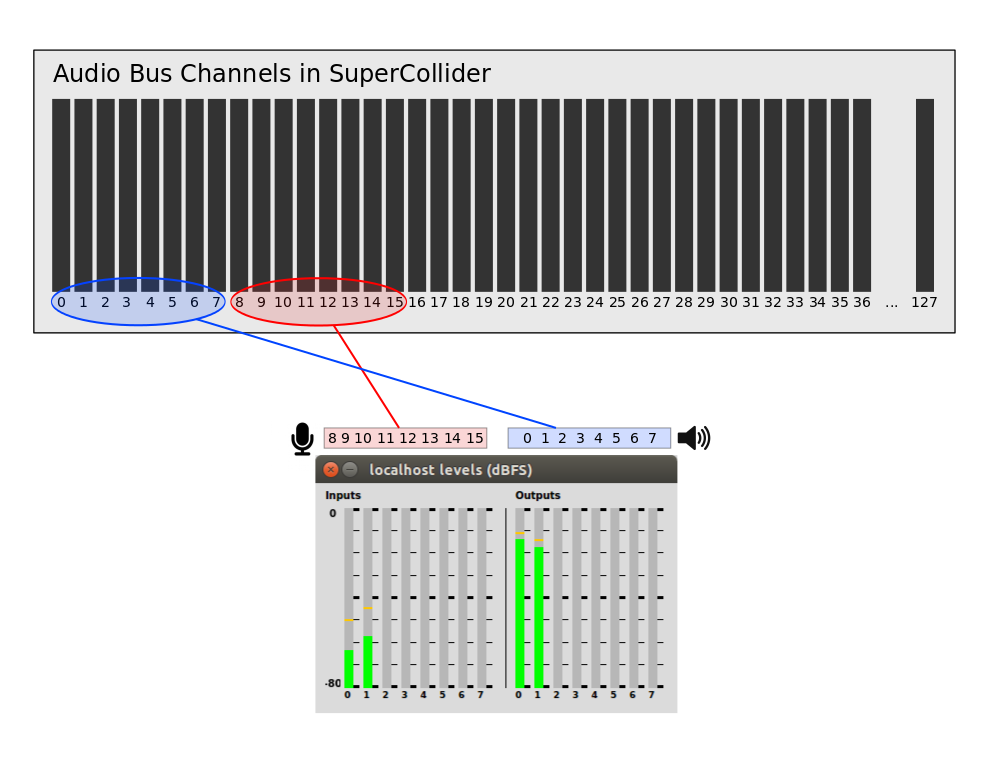
\includegraphics[scale=0.4]{fig-audio-bus.png}}
\caption{Canais de áudio e a janela Meter no SC.}
\label{fig:audio-bus}
\end{figure}

Pressione [ctrl+M] para abrir a janela Meter ("medidor"). Ela mostra os níveis de todas as entradas e saídas. A figura \ref{fig:audio-bus} mostra uma captura de tela dessa janela e sua correspondência com os canais padrão do SuperCollider. No SC, canais de áudio são numerados de 0 a 127. Os primeiros oito (0-7) são por definição reservados para serem os canais de saída da sua placa de com. Os próximos oito (8-15) são reservados para as entradas da sua placa de som. Todos os outros (16 a 127) estão livres para serem utilizados de qualquer forma que se queira, por exemplo, quando você precisa rotear sinais de áudio de uma UGen para outra.

\subsection{\texttt{Out} and \texttt{In} UGens}

Agora experimente a seguinte linha de código:

\begin{lstlisting}[style=SuperCollider-IDE, basicstyle=\scttfamily\footnotesize]
{Out.ar(1, SinOsc.ar(440, 0, 0.1))}.play; // canal direito
\end{lstlisting}

A UGen \texttt{Out} UGen cuida do roteamento de sinais para canais específicos.

O primeiro argumento para \texttt{Out} é o canal de destino, isto é, para onde você quer que o sinal vá. No exemplo acima, o número \texttt{1} significa que queremos mandar o sinal para o canal 1, que é o canal direito da sua placa de som.

O segundo argumento de \texttt{Out.ar} é o sinal de fato que você quer "escrever" neste canal. Pode ser uma única UGen, ou uma combinação de UGens. No exemplo, é somente uma onda senoidal. Você deve ouvi-la somente no seu alto-falante direito (ou seu ouvido direito, se estiver usando fones de ouvido).

Com a janela Meter aberta e visível, vá ao código e mude o primeiro argumento de \texttt{Out.ar}: tente qualquer número entre 0 e 7. Observe os medidores. Você verá que o sinal vai para qualquer lugar que você mandar.

\bigskip
\todo[inline, color=green!40]{DICA: É bastante provável que você tenha uma placa de som que só pode tocar dois canais (esquerdo e direito), então você somente escutará a senoide quando mandá-la para o canal 0 ou 1. Se você enviá-la para outros canais (3 a 7), você ainda verá o medidor correspondente mostrando o sinal: o SC está de fato mandando som para aquele canal, mas a menos que você tenha uma placa de som de 8 canais, você não poderá ouvir a saída dos canais 3-7.}
\bigskip

Um exemplo simples de um canal de áudio sendo usado para um efeito é mostrado abaixo.

\begin{lstlisting}[style=SuperCollider-IDE, basicstyle=\scttfamily\footnotesize]
// iniciar o efeito
f = {Out.ar(0, BPF.ar(in: In.ar(55), freq: MouseY.kr(1000, 5000), rq: 0.1))}.play;
// iniciar a fonte sonora
n = {Out.ar(55, WhiteNoise.ar(0.5))}.play;
\end{lstlisting}

A primeira linha declara um sintetizador (armazenado na variável \texttt{f}), consistindo em uma UGen de filtro (Band Pass Filter: "filtro passa-banda"). Um filtro passa-banda aceita qualquer som como entrada e \emph{elimina todas as frequências exceto a região de frequência que você quer deixar passar}. \texttt{In.ar} é a UGen que usamos para ler de um canal de áudio. Portanto, com \texttt{In.ar(55)} sendo utilizado como entrada para o \texttt{BPF}, qualquer som que mandarmos para o canal 55 passará pelo filtro passa-banda. Note que o primeiro sintetizador, em um primeiro momento, não produz som algum: quando você roda a primera linha, o canal 55 continua vazio. Ele somente produzirá som quando mandarmos algum audio para o canal 55, que é o que acontece na segunda linha.

A segunda linha cria um sintetizador e o armazena na variável \texttt{n}. Este sintetizador simplesmente gera ruído branco, e o envia \emph{não diretamente para os alto-falantes, mas sim para o canal de audio 55}. Este é precisamente o canal que nosso sintetizador de filtro está escutando, então assim que você rodar a segunda linha, você deve começar a ouvir o ruído branco sendo filtrado pelo sintetizador \texttt{f}.

Em resumo, o roteamento tem a seguinte configuração: 

\begin{center}
\emph{sintetizador de ruído} $\rightarrow$ \emph{canal 55} $\rightarrow$ \emph{sintetizador de filtro}
\end{center}

A ordem de execução é importante. O exemplo anterior não funcionará se você não rodar a fonte \emph{antes} do efeito. Isso será discutido em mais detalhe na seção \ref{sec:order-of-execution}, "Ordem de Execução".

Uma última coisa: quando em exemplos anteriores você escreveu sintetizadores como \texttt{\{SinOsc.ar(440)\}.play}, internamente o SC estava de fato executando \texttt{\{Out.ar(0, SinOsc.ar(440))\}.play}: ele assume que você queria mandar som para o canal 0, então ele automaticamente embute a primeira UGen em uma UGen \texttt{Out.ar(0, ...)}. Na realidade, há mais algumas coisas acontecendo nos bastidores, mas voltaremos a isso mais tarde (seção \ref{sec:synthdef}).
